% ============================ Enrico Ribiani 16-03-2021 ====================================================================
% Base per i documenti  
\documentclass[12pt]{article}
% ------------ pacchetti necessari ----------------
\usepackage[a4paper, total={6in, 8in},margin=1in]{geometry} % formattazione decente della pagina
\usepackage{graphicx}                            % need for figure
\usepackage{amsmath}
\usepackage{amsfonts}                            % if you want the fonts
\usepackage{amssymb}                             % if you want extra symbols
\usepackage{graphicx}  
\renewcommand{\figurename}{Figure}  
\renewcommand{\contentsname}{Index}                        % need for figures
\usepackage{mathptmx}
\usepackage{float}                               % serve per mettere tabelle e immagini dove si vuole 
\usepackage[utf8]{inputenc}
\usepackage{textcomp}
\usepackage[hang,flushmargin,bottom]{footmisc}   % footnote format
\usepackage{fancyhdr, lastpage}
\usepackage{titlesec}
\usepackage[table,dvipsnames]{xcolor}
%\pagestyle{fancy}
%\renewcommand{\headrulewidth}{0pt}
%\renewcommand*\contentsname{Indice}
\titleformat{\section}{\normalsize\bfseries}{\thesection.}{1em}{}	% required for heading numbering style
\titleformat*{\section}{\Large\bfseries}
\titleformat*{\subsection}{\large\bfseries}
%\usepackage{siunitx}
%\usepackage{tikz}
\usepackage{circuitikz}
%\usepackage[siunitx]{circuitikz}
\usepackage{multirow}
\usepackage{tikz}
\usepackage{amsmath}
\usepackage{shorttoc}
\usetikzlibrary{angles,quotes}
\usepackage{placeins}

\usepackage{wasysym}
%===================links=================
\usepackage{hyperref}
\hypersetup{
    colorlinks=true,
    linkcolor=darkgray,
    filecolor=Green,      
    urlcolor=Cyan,
    pdftitle={SAMPLE},
    pdfpagemode=FullScreen,
    }

	\usepackage[demo]{graphicx}
\usepackage{caption}
\usepackage{subcaption}
%===================inizio pagina del titolo=================
\begin{document}
\pagenumbering{gobble}
\begin{titlepage}
	\begin{center}
		% ------------------ inizio immagine logo ----------
		\begin{figure}
			\centering
			
\includegraphics[scale=1.2]{~/Documenti/latec/logo.png}
			\label{fig:logo}
		\end{figure}
		% ------------------ fine immagine logo ----------
		% ------------------ fine immagine logo ----------
		-------------------------------------------------------------------------------------\\
		\vspace{2\baselineskip}
		\large $5^a$AUB\\
		\large Enrico Ribiani\\
		\large Nicolò Cellana\\
		\large Marco Ciola\\


		\vfill

		\Huge{\textbf{Photovoltaic panels measures}}\\
		\vfill

		\LARGE{$5^{th}$ report}\\
		\vfill
		\large{19-05-2023}
	\end{center}
	%=============== fine pagina titolo ===============
\end{titlepage}
\tableofcontents
\newpage
\pagenumbering{arabic}
\setcounter{page}{1}
\section{Introduction}
This report will illustrate the laboratory experience, carried out on 12 May 2023, focused on the study of
photovoltaic panels.\\
The collection of data took place inside the courtyard of the ITT Buonarroti (TN), during the
afternoon with suitable weather conditions,direct sun exposure, positioning the panels appropriately with an
inclination of approximately 37° facing northwest.\\
We underline how the duration of the collection of the values could slightly compromise the reliability of
the measurements, this is mainly due to the variable exposure conditions of the panels to solar radiation
over time and the variation of temperature of the panels that reached 44°C starting from around 28°C.\\
The report also contains the analisys of the data collected, the power output and an approximative extimation
of the radiation.\\
\section{Pv panels theory}

\section{Request}
The objective of this activity was to survey the characteristics of three photovoltaic panels made with different
technologies and from their comparison derive an estimate of the incident energy.\\
In order to achieve this we collected the current and the tension generated by the thre
Using the voltamperometric measurements collected under the same condition and in different load configurations we were asked to trace the graph of the
panels characteristics.\\
Besides that
\section{Wiring diagrams}
\begin{figure}[ht]
	\centering
	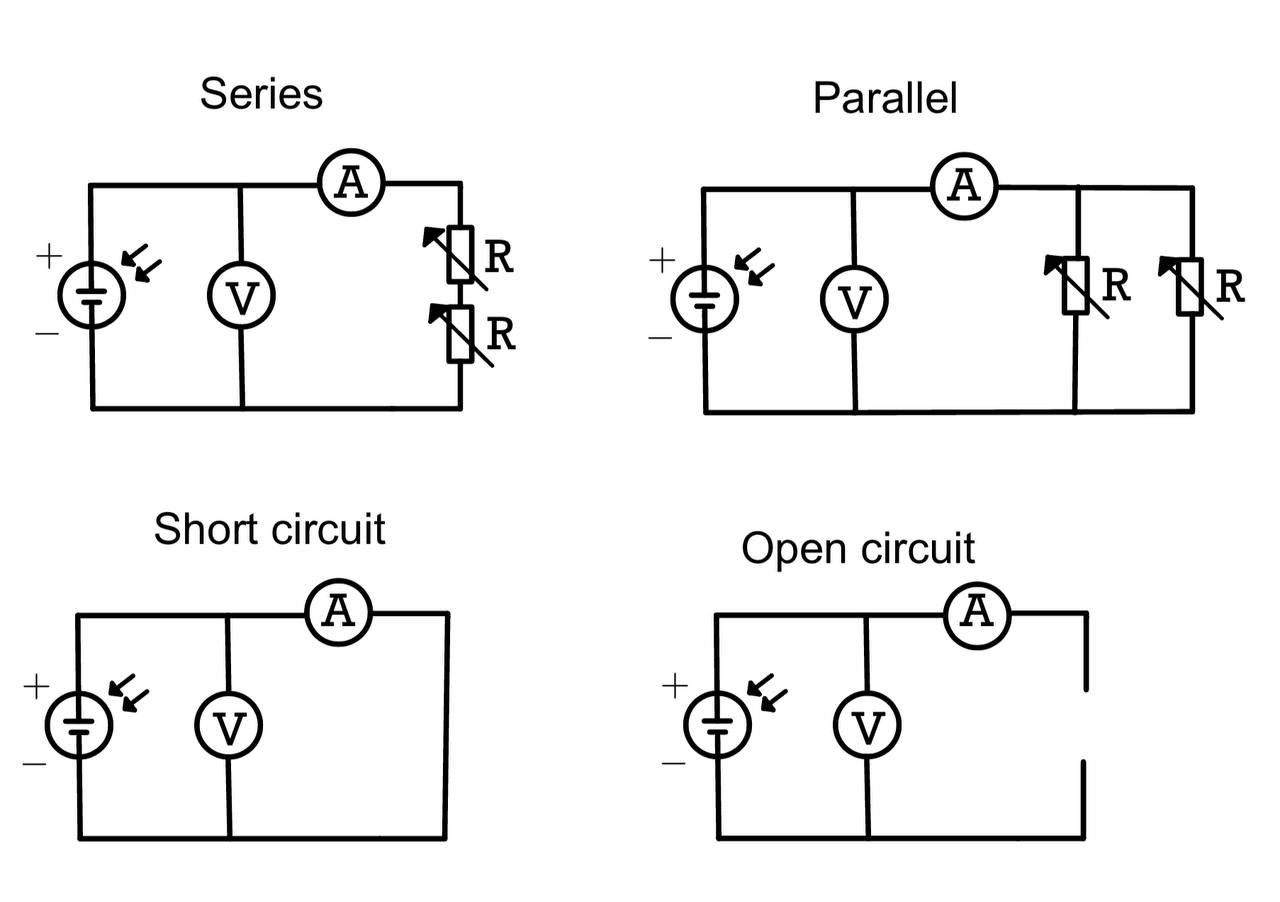
\includegraphics[scale=0.2]{schema.jpg}
\end{figure}
\subsection{Equipment}
\begin{itemize}
    \item Connection Wires
    \item Benq PM245P00
    \item Panda 60 cells
    \item Sharp NA-E135L5 series
    \item Rheostat  $200\Omega$ and 2,5A maximum
    \item 2x Multimeter
    \end{itemize}

\section{Procedure}
\section{Tables}
\subsection{Benq PM245P00}
\begin{table}[h]
	\centering
	\begin{tabular}{|p{2cm}|p{2cm}|p{2cm}|}
		\hline
		\rowcolor{RoyalBlue!80} Voltage [V] & Current [A] & Power [W] \\
		\hline
		\rowcolor{Cerulean!70} 33,7         & 0           & 0         \\
		\hline
	\end{tabular}
	\caption{Open circuit}
	\label{tab:my_label}
\end{table}

\begin{table}[h]
	\centering
	\begin{tabular}{|p{2cm}|p{2cm}|p{2cm}|}
		\hline
		\rowcolor{Green!80} Voltage [V] & Current [A] & Power [W] \\
		\hline
		\rowcolor{LimeGreen!70} 33,6    & 0,007       & 0,2       \\
		\hline
		\rowcolor{YellowGreen!70} 33,4  & 0,009       & 0,3       \\
		\hline
		\rowcolor{LimeGreen!70} 33,2    & 0,11        & 3,7       \\
		\hline
		\rowcolor{YellowGreen!70} 33,2  & 0,15        & 5,0       \\
		\hline
	\end{tabular}
	\caption{Series}
	\label{tab:my_label}
\end{table}

\begin{table}[h]
	\centering
	\begin{tabular}{|p{2cm}|p{2cm}|p{2cm}|}
		\hline
		\rowcolor{RedOrange!80} Voltage [V] & Current [A] & Power [W] \\
		\hline
		\rowcolor{Peach!70} 33,2            & 0,3         & 10,0      \\
		\hline
		\rowcolor{Melon!70} 33              & 0,36        & 11,9      \\
		\hline
		\rowcolor{Peach!70} 33              & 0,41        & 13,5      \\
		\hline
		\rowcolor{Melon!70} 33              & 0,46        & 15,18     \\
		\hline
		\rowcolor{Peach!70} 33              & 0,53        & 17,5      \\
		\hline
		\rowcolor{Melon!70} 32,9            & 0,6         & 19,7      \\
		\hline
		\rowcolor{Peach!70} 32,8            & 0,7         & 23,0      \\
		\hline
		\rowcolor{Melon!70} 32,6            & 0,86        & 28,0      \\
		\hline
		\rowcolor{Peach!70} 32,5            & 1,18        & 38,4      \\
		\hline
		\rowcolor{Melon!70} 32,1            & 1,77        & 56,8      \\
		\hline
		\rowcolor{Peach!70} 30,1            & 4,08        & 122,8     \\
		\hline
		\rowcolor{Melon!70} 29              & 4,26        & 123,5     \\
		\hline
	\end{tabular}
	\caption{Parallel}
	\label{tab:my_label}
\end{table}

\begin{table}[!h]
	\centering
	\begin{tabular}{|p{2cm}|p{2cm}|p{2cm}|}
		\hline
		\rowcolor{Red!80} Voltage [V] & Current [A] & Power [W] \\
		\hline
		\rowcolor{Red!60} 0           & 5,45        & 0         \\
		\hline
	\end{tabular}
	\caption{Short circuit}
	\label{tab:my_label}
\end{table}

\FloatBarrier
\subsection{Panda 60 cells}
\begin{table}[!h]
	\centering
	\begin{tabular}{|p{2cm}|p{2cm}|p{2cm}|}
		\hline
		\rowcolor{RoyalBlue!80} Voltage [V] & Current [A] & Power [W] \\
		\hline
		\rowcolor{Cerulean!70}    35,5      & 0           & 0         \\
		\hline
	\end{tabular}
	\caption{Open circuit}
	\label{tab:my_label}
\end{table}

\begin{table}[!h]
	\centering
	\begin{tabular}{|p{2cm}|p{2cm}|p{2cm}|}
		\hline
		\rowcolor{Green!80} Voltage [V]  & Current [A] & Power [W] \\
		\hline
		\rowcolor{LimeGreen!70}    34,9  & 0,07        & 0,2       \\
		\hline
		\rowcolor{YellowGreen!70}   35   & 0,08        & 2,8       \\
		\hline
		\rowcolor{LimeGreen!70}    35,1  & 0,09        & 3,2       \\
		\hline
		\rowcolor{YellowGreen!70}   35,1 & 0,1         & 3,5       \\
		\hline
		\rowcolor{LimeGreen!70}     35,2 & 0,11        & 3,9       \\
		\hline
	\end{tabular}
	\caption{Series}
	\label{tab:my_label}
\end{table}

\begin{table}[!h]
	\centering
	\begin{tabular}{|p{2cm}|p{2cm}|p{2cm}|}
		\hline
		\rowcolor{RedOrange!80} Voltage [V] & Current [A] & Power [W] \\
		\hline
		\rowcolor{Peach!70}       34,8      & 0,3         & 10,4      \\
		\hline
		\rowcolor{Melon!70}        34,8     & 0,34        & 11,8      \\
		\hline
		\rowcolor{Peach!70}         34,8    & 0,36        & 12,5      \\
		\hline
		\rowcolor{Melon!70}        34,7     & 0,41        & 14,2      \\
		\hline
		\rowcolor{Peach!70}        34,7     & 0,45        & 15,6      \\
		\hline
		\rowcolor{Melon!70}          34,6   & 0,54        & 18,7      \\
		\hline
		\rowcolor{Peach!70}         34,5    & 0,7         & 24,2      \\
		\hline
		\rowcolor{Melon!70}          34,4   & 0,94        & 32,3      \\
		\hline
		\rowcolor{Peach!70}           34,2  & 1,18        & 40,4      \\
		\hline
		\rowcolor{Melon!70}         33,8    & 1,74        & 58,8      \\
		\hline
		\rowcolor{Peach!70}           33    & 2,8         & 92,4      \\
		\hline
		\rowcolor{Melon!70}           32,5  & 3,26        & 106,0     \\
		\hline
		\rowcolor{Peach!70}           32    & 3,8         & 121,6     \\
		\hline
		\rowcolor{Melon!70}           31,9  & 3,97        & 126,6     \\
		\hline
	\end{tabular}
	\caption{Parallel}
	\label{tab:my_label}
\end{table}

\begin{table}[!h]
	\centering
	\begin{tabular}{|p{2cm}|p{2cm}|p{2cm}|}
		\hline
		\rowcolor{Red!80} Voltage [V] & Current [A] & Power [W] \\
		\hline
		\rowcolor{Red!60} 0           & 6,68        & 0         \\
		\hline
	\end{tabular}
	\caption{Short circuit}
	\label{tab:my_label}
\end{table}
\FloatBarrier
\subsection{Sharp NA-E135L5 series}
\begin{table}[!h]
	\centering
	\begin{tabular}{|p{2cm}|p{2cm}|p{2cm}|}
		\hline
		\rowcolor{RoyalBlue!80} Voltage [V] & Current [A] & Power [W] \\
		\hline
		\rowcolor{Cerulean!70}     56,9     & 0           & 0         \\
		\hline
	\end{tabular}
	\caption{Open circuit}
	\label{tab:my_label}
\end{table}

\begin{table}[!h]
	\centering
	\begin{tabular}{|p{2cm}|p{2cm}|p{2cm}|}
		\hline
		\rowcolor{Green!80} Voltage [V]  & Current [A] & Power [W] \\
		\hline
		\rowcolor{LimeGreen!70}   56,1   & 0,12        & 6,7       \\
		\hline
		\rowcolor{YellowGreen!70}  56    & 0,14        & 7,8       \\
		\hline
		\rowcolor{LimeGreen!70}     55,9 & 0,17        & 9,5       \\
		\hline
		\rowcolor{YellowGreen!70}  55,8  & 0,22        & 12,3      \\
		\hline
		\rowcolor{LimeGreen!70}    55,6  & 0,29        & 16,1      \\
		\hline
		\rowcolor{YellowGreen!70} 55,1   & 0,48        & 26,4      \\
		\hline
	\end{tabular}
	\caption{Series}
	\label{tab:my_label}
\end{table}

\begin{table}[!h]
	\centering
	\begin{tabular}{|p{2cm}|p{2cm}|p{2cm}|}
		\hline
		\rowcolor{RedOrange!80} Voltage [V] & Current [A] & Power [W] \\
		\hline
		\rowcolor{Peach!70}   55,3          & 0,51        & 28,2      \\
		\hline
		\rowcolor{Melon!70}     55,2        & 0,56        & 31,0      \\
		\hline
		\rowcolor{Peach!70}      55,2       & 0,63        & 34,8      \\
		\hline
		\rowcolor{Melon!70}        54,9     & 0,71        & 39,0      \\
		\hline
		\rowcolor{Peach!70}        54,5     & 0,81        & 44,1      \\
		\hline
		\rowcolor{Melon!70}    54,2         & 0,93        & 50,4      \\
		\hline
		\rowcolor{Peach!70}    53,3         & 1,13        & 60,2      \\
		\hline
		\rowcolor{Melon!70}     52,2        & 1,37        & 71,5      \\
		\hline
		\rowcolor{Peach!70}      50,2       & 1,72        & 86,3      \\
		\hline
		\rowcolor{Melon!70}       42,8      & 2,2         & 94,2      \\
		\hline
		\rowcolor{Peach!70}        22,8     & 2,34        & 53,4      \\
		\hline
	\end{tabular}
	\caption{Parallel}
	\label{tab:my_label}
\end{table}

\begin{table}[!h]
	\centering
	\begin{tabular}{|p{2cm}|p{2cm}|p{2cm}|}
		\hline
		\rowcolor{Red!80} Voltage [V] & Current [A] & Power [W] \\
		\hline
		\rowcolor{Red!60} 0           & 2,45        & 0         \\
		\hline
	\end{tabular}
	\caption{Short circuit}
	\label{tab:my_label}
\end{table}
\vfill
\newpage
\FloatBarrier

\section{Graphs}
\subsection{Benq PM245P00}
%\begin{figure}[!ht]
%	\centering
	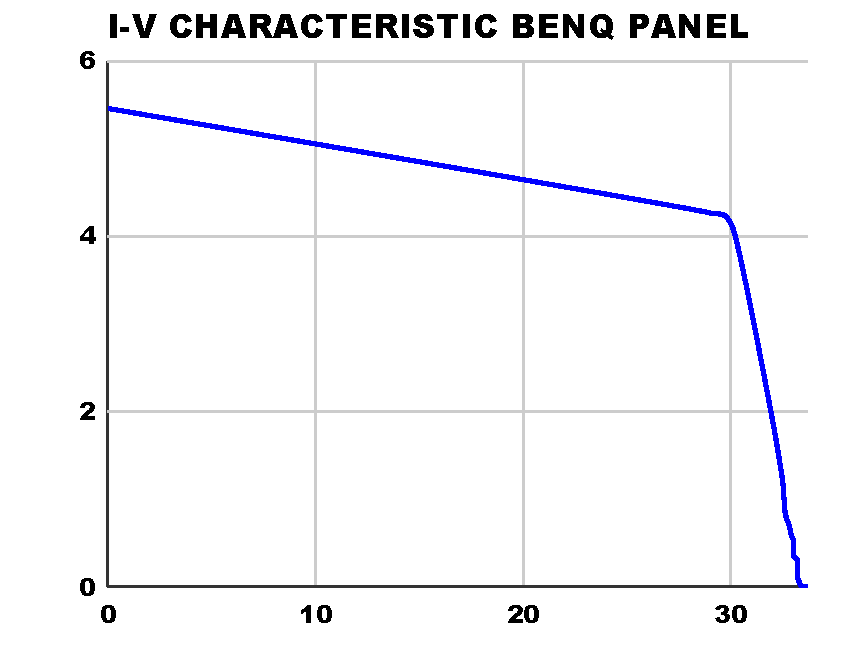
\includegraphics[scale=0.6]{benq-iv.pdf}
%\end{figure}
\subsection{Panda 60 cells}
%\begin{figure}[!h]
%	\centering
	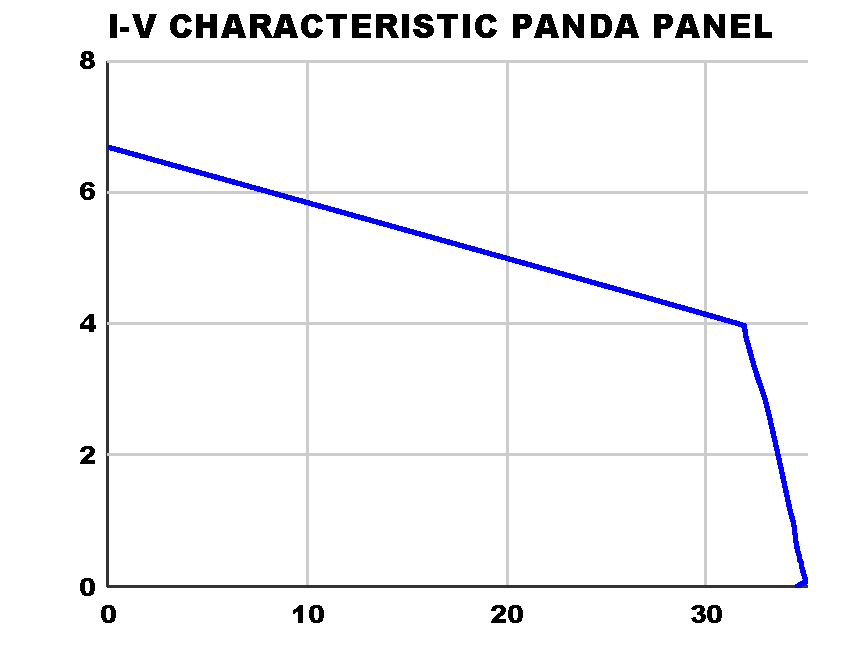
\includegraphics[scale=0.6]{panda-iv.pdf}
%\end{figure}
\subsection{Sharp NA-E135L5 series}
%\begin{figure}[!h]
%	\centering
	%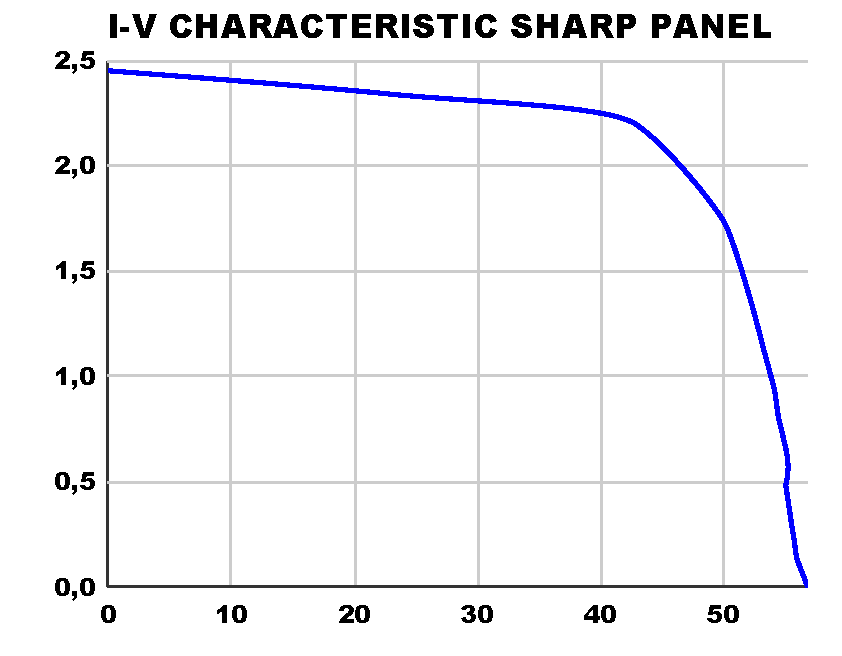
\includegraphics[scale=0.6]{sharp-iv.pdf}
%\end{figure}
\begin{figure}
	\centering
	\begin{subfigure}{.5\textwidth}
	  \centering
	  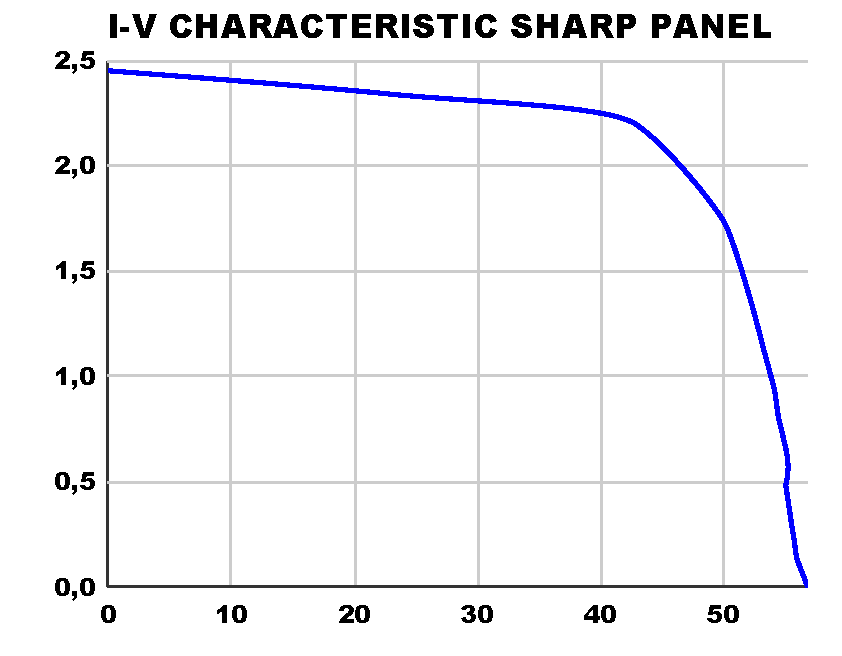
\includegraphics[width=.4\linewidth]{sharp-iv.pdf}
	  \caption{Our graph}
	  \label{fig:sub1}
	\end{subfigure}%
	\begin{subfigure}{.5\textwidth}
	  \centering
	  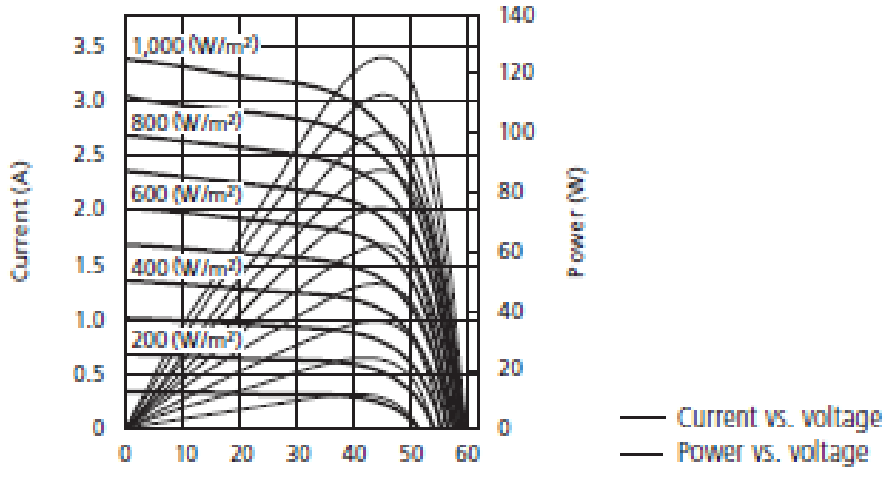
\includegraphics[width=.4\linewidth]{sharp-data-iv.png}
	  \caption{Datasheet graph}
	  \label{fig:sub2}
	\end{subfigure}
	\end{figure}
	
	\begin{figure}
\section{Data analisys}
\subsection{Radiation}
\section{Conclusions}

\end{document}